\chapter{Livello Trasporto}
\section{Introduzione}
Il livello di trasporto estende il servizio di consegna del protocollo IP tra due host terminali a un servizio di consegna per due processi applicativi in esecuzione sugli host.
Inoltre, aggiunge alcune funzionalità, come il controllo di errori e il multiplexing/demultiplexing dei messaggi fra processi.
I protocolli principali sono due:
\begin{enumerate}
    \item \textbf{TCP (Trasmission Control Protocol).}
    \item \textbf{UDP (User Datagram Procotol).}
\end{enumerate}

\begin{figure}[!htb]
    \centering
    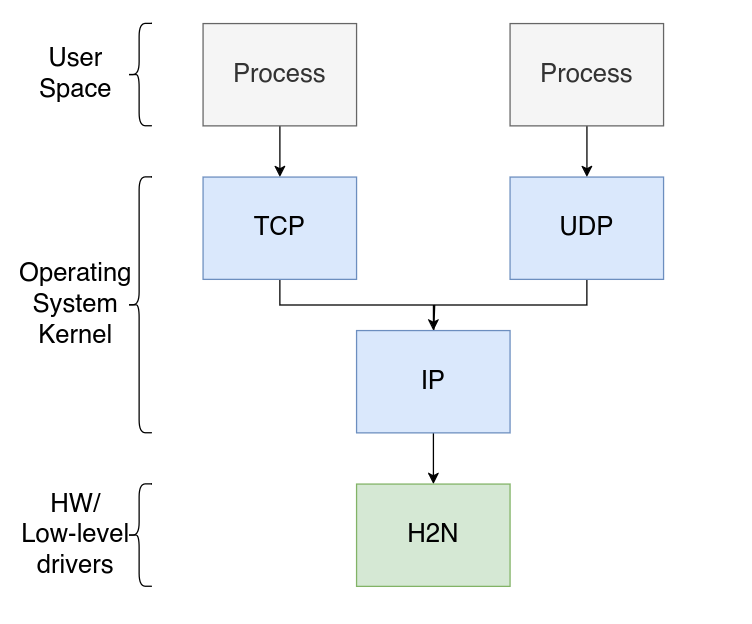
\includegraphics[width=0.5\linewidth]{Images/livello_trasporto/Trasporto.png}
    \caption{Schema comunicazione con protocolli e livelli.}
\end{figure}

\subsection{Multiplexing e Demultiplexing}
Il protocollo IP non trasferisce dati tra i processi applicativi in esecuzione sui nodi finali, questo è compito dei protocolli di trasporto:
\begin{itemize}
    \item \textbf{Multiplexing:} creazione di segmenti derivanti da messaggi di diversi processi applicativi, avviene sul nodo sorgente.
    \item \textbf{Demultiplexing:} ogni segmento del livello di trasporto ha un campo contenente le informazioni utilizzate per determinare a quale processo il segmento deve essere consegnato, avviene del nodo di destinazione.
\end{itemize}
I protoclli UDP e TCP aggiungo per fare questo due campi nell'header del segmento:
\begin{enumerate}
    \item \textbf{Numero di porta del mandante.}
    \item \textbf{Numero di porta del destinatario.}
\end{enumerate}

\begin{boxDef}
\textbf{\textcolor{brown}{Porta:}} strumento utilizzato per il multiplexing/demulultiplexing per identificare in modo \textbf{univico} i \textbf{processi} e che permette di eseguire connessioni multiple sullo stesso host. Le porte si dividono in tre categorie:
\begin{enumerate}
    \item \textbf{Porte Well-Knwon:} da 0 a 1023.
    \item \textbf{Porte Registrate:} da 1024 a 49151.
    \item \textbf{Porte Dinamiche o Private:} da 49152 a 65535.
\end{enumerate}
\end{boxDef}
Due processi client, che comunicano con lo stesso servizio applicativo, sono sempre distinti in base alla tupla:
\[
\text{[(\textbf{\textcolor{blue}{Source IP}}, \textbf{\textcolor{blue}{Source Port}}), (\textbf{\textcolor{red}{Destination IP}}, \textbf{\textcolor{red}{Destination Port}})]}
\]

\section{Protocollo UDP}
UDP (User Datagram Protocol) è un protocollo di trasporto molto leggere, partendo dall'\textbf{IP Datagram}, aggiunge alcuni header:

\begin{figure}[!htb]
    \centering
    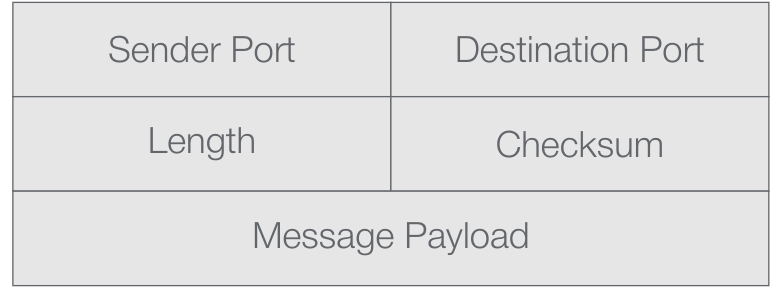
\includegraphics[width=0.5\linewidth]{Images/livello_trasporto/UDP_header.png}
    \caption{Segmento UDP.}
\end{figure}

In particolare:
\begin{itemize}
    \item \textbf{Numero di porta sorgente} (16 bit). 
    \item \textbf{Numero di porta di destinazione} (16 bit).
    \item \textbf{Lunghezza} (16 bit): header + data, dove l'header è sempre 8 byte.
    \item \textbf{Checksum} (16 bit).
\end{itemize}

\subsection{Campo Checksum}
Questo campo è stato aggiungo perchè non tutte le connessioni a livello H2N hanno un controllo dell'errore e inoltre, il controllo dell'errore con checksum a livello IP controlla solo il datagram IP.
Quindi, a livello di trasporto, non ci sarebbe stato nessun modo di avere un ripristino dall'errore.
\\
Nel pratico:
\begin{itemize}
    \item \textbf{Sorgente:} tratta il contenuto del segmento come una sequenza di numeri interi a 16 bit, somma il contenuto dei segmenti in complemento a uno e invia il valore del checksum nel campo del segmento UDP.
    \item \textbf{Desrinatario:} calcola il checksum del segmento ricevuto e verifica se il valore del checksum calcolato è uguale a quello ricevuto.
\end{itemize}

\vspace*{0.02\textheight}
\textbf{ESEMPIO:}
\vspace*{0.01\textheight}
\begin{center}
    \begin{tabular}{ c | c }
        \hline
        \textbf{Word 1} & 0110011001100110 \\
        \textbf{Word 2} & 0101010101010101 \\
        \textbf{Word 3} & 0000111100001111 \\
        \hline
        \textbf{Somma} & 1100101011001010 \\
        \hline
        \textbf{Complemento a 1} & 0011010100110101 \\
        \hline
    \end{tabular}
\end{center}
Il destinatario calcola il proprio checksum del segmento UDP, senza calcolare il complemento a uno:
\begin{itemize}
    \item \textbf{OK:} checksum destinazione + checksum UDP = 1111111111111111.
    \item \textbf{ERRORE:} Checksum destinazione + checksum UDP != 1111111111111111.
\end{itemize}

\section{Protocollo TCP}
Il protocollo TCP fornisce un livello di trasporto affidabile e orientato alla connessione. Ha alcuni servizi aggiuntivi rispetto a UDP:
\begin{itemize}
    \item \textbf{Orientato alla connessione:} include le fasi di  stabilimento, utilizzo e chiusura della connessione.
    \item \textbf{Orientato al flusso di dati:} considera il flusso di dati dall'host mittente al destinatario.
    \item \textbf{Trasferimento con buffer:} i dati vengono memorizzati in un buffer e quindi inseriti in un pacchetto quando il buffer è pieno.
    \item \textbf{Connessione full-duplex (bidirezionale):} una volta stabilita la connessione, è possibile il trasferimento simultaneo in entrambe le direzioni della connessione.
\end{itemize}

\subsection{Affidabilità}
Affidabile significa che TCP gestisce il trasferimento di un flusso di dati con la sequenza corretta (ACK + timeout + ritrasmissione):
\begin{itemize}
    \item Ogni trasmissione riuscita viene notificata (\textbf{ACK}) dall'host ricevente.
    \item Se l'host mittente non riceve una conferma entro un intervallo di tempo predefinito (\textbf{timeout}), il mittente ritrasmette i dati.
    \item Gli \textbf{ACK} e le \textbf{ritrasmissioni} dovute a eventuali perdite vengono gestite in modo trasparente rispetto al processo applicativo.
\end{itemize}

\subsection{Trasferimento con buffer}
Per risolvere molti dei problemi evidenziati sopra, il livello TCP deve necessariamente utilizzare un buffer per evitare:
\begin{itemize}
    \item Invio asincrono dei dati rispetto al processo applicativo.
    \item Tempi di trasmissione differenti.
    \item Capacità di invio e ricezione differenti.
    \item Segmenti persi o fuori sequenza.
\end{itemize}
Inoltre, il protocollo TCP ha altri due compiti fondamentali:
\begin{enumerate}
    \item \textbf{Controllo della congestione:} l'host mittente deve ridurre la velocità di trasmissione dei pacchetti quando la rete è congestionata.
    \item \textbf{Controllo del flusso:} l'host mittente non deve sovraccaricare l'host ricevente.
\end{enumerate}

\begin{figure}[!htb]
    \centering
    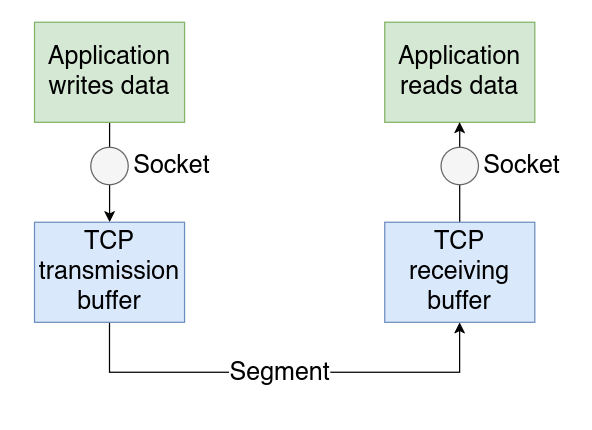
\includegraphics[width=0.5\linewidth]{Images/livello_trasporto/TCP_buffer.png}
    \caption{Esempio di utilizzo del buffer TCP.}
\end{figure}

Un'applicazione può anche indicare a TCP di inviare i dati presenti nel buffer, senza attendere che quest'ultimo sia pieno.

\section{TCP Segment}
L'insieme di dati che il livello TCP richiede di trasferire al livello IP è chiamato segmento TCP ed è formato da una parte di header e da una parte di byte di dati.

\begin{figure}[!htb]
    \centering
    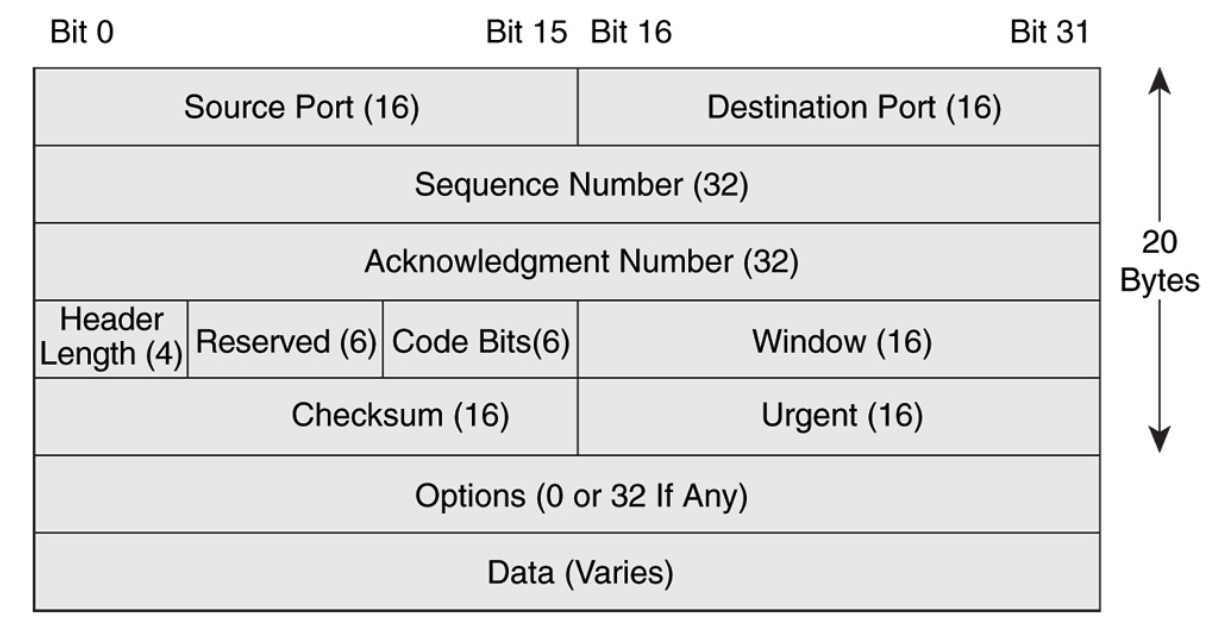
\includegraphics[width=0.7\linewidth]{Images/livello_trasporto/TCP_segment.png}
    \caption{Esempio di utilizzo del buffer TCP.}
\end{figure}

Nello specifico:
\begin{itemize}
    \item \textbf{Porta sorgente} (16 bit).
    \item \textbf{Porta di destinazione} (16 bit).
    \item \textbf{Sequence number} (32 bit): sequence number relativo al flusso di byte trasmesso.
    \item \textbf{Acknowledgment number} (32 bit): ACK relativo al sequence number del flusso di byte ricevuto.
    \item \textbf{Lunghezza dell'header} (4 bit): lunghezze in multipli di 32 bit dell'header, se non ha opzioni è sempre 20 byte.
    \item \textbf{Reserved} (6 bit): riservato per usi futuri.
    \item \textbf{Code bit} (6 bit): usato per le varie flag:
    \begin{itemize}
        \item URG: dati segnati come urgenti dal layer applicativo.
        \item ACK: valore dell'ACK è valido.
        \item PSH: i dati devono essere passati all'applicazione subito.
        \item SYN, FIN, RST: usati per stabilire, chiudere o interropere una connessione.
    \end{itemize}
    \item \textbf{Dimensione della finestra} (16 bit): indica il numero di byte che il destinatario è disposto ad accettare.
    \item \textbf{Checksum} (16 bit): controllo dell'integrità come nell'UDP.
    \item \textbf{Urgent} (16 bit): puntatore alla fine dei dati urgenti.
    \item \textbf{Opzioni} (0-32 bit): campi opzionali di varie dimensioni (come MSS - maximun segment size).
    \item \textbf{Padding di zeri} se necessario.
\end{itemize}
Alcuni esempi di dati urgenti posso essere i segnali come \textit{Ctrl + Z} o \textit{Ctrl + C}, in modo che possano arrivare immediatamente. Quando vengono ricevuti, saltano direttamente lo stream di byte e arrivano all'applicazione. Sono posizionati all'inzio del segmento, per questo il puntatore Urgent punta alla loro fine.

\newpage
\section{Inizializzare e chiudere una connessione TCP}
Nel protocollo TCP, il mittente e il destinatario stabiliscono la connessione e inizializzano le variabili dei segmenti prima di iniziare il trasferimento, utilizzando un modello \textbf{client/server}. \\
Per stabilire una connessione il client invia un segmento particolare, dove imposta il campo \textbf{SYN} a 1, al server. Deve contenere:
\begin{itemize}
    \item La porta del server.
    \item L'\textbf{ISN (Initial Sequence Number)} del client, un numero a 32 bit pseudo randomico, da cui inizierà la numerazione.
    \item L'\textbf{MRW (Maximum Receive Window)}, ossia il numero di byte che il client può ricevere nel buffer.
    \item L'\textbf{MSS (Maximum Segment Size)}, la grandezza massima del segmento, anche se non sempre è inviata.
\end{itemize}
Questo segmento TCP non contiene nessun dato, ma solo l'header.
Il server, al sua volta, risponderà con un segmento con \textbf{SYN} a 1 e con gli stessi campi, ma con i valori riferiti a lui e con un ACK con valore dell'\textbf{ISN} del client aumentato di uno. Infine, il client risponderà con un \textbf{ACK} del valore dell'\textbf{ISN} del server aumentato di uno.

\begin{figure}[!htb]
    \centering
    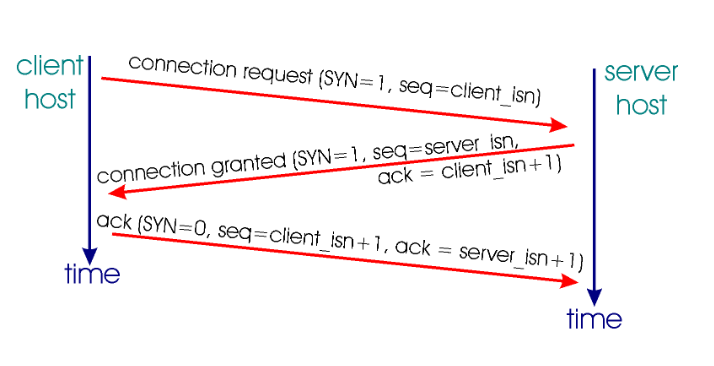
\includegraphics[width=0.7\linewidth]{Images/livello_trasporto/Three-way-hand.png}
    \caption{Esempio di three-way-handshaking.}
\end{figure}

Per chiudere una connessione in modo pulito, il client deve mandare un segmento con il campo \textbf{FIN} a 1 al server, il quale dopo aver risposto al client con un \textbf{ACK}, chiude la connessione lato client e invia a sua volta un segmento con campo \textbf{FIN} a 1 al client. Infine, il client dopo aver ricevuto il \textbf{FIN} del server gli invia un \textbf{ACK}. Il server appena riceve l'\textbf{ACK} chiude la connessione, il client la chiude dopo un tempo di timeout. \\
Un altro modo per interropere una connessione è impostare il campo \textbf{RST} a 1, questo farà si che l'altro nodo chiuda immediatamente la connessione e che tutte le risorse vengano liberate.

\begin{figure}
    \begin{minipage}{.45\linewidth}
        \centering
        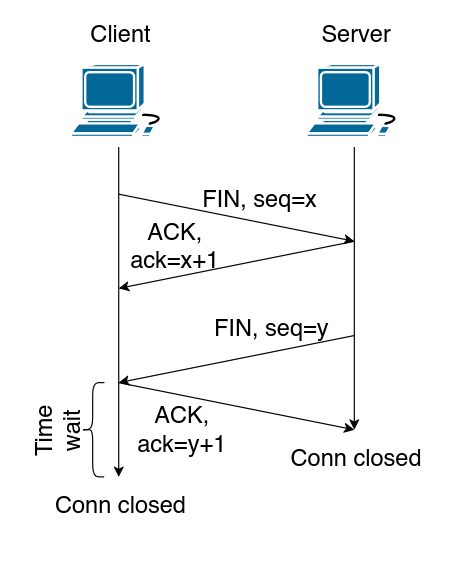
\includegraphics[width=0.6\linewidth]{Images/livello_trasporto/FIN.png}
        \caption{Chiusura pulita di una connessione.}
    \end{minipage}
    \begin{minipage}{.45\linewidth}
        \centering
        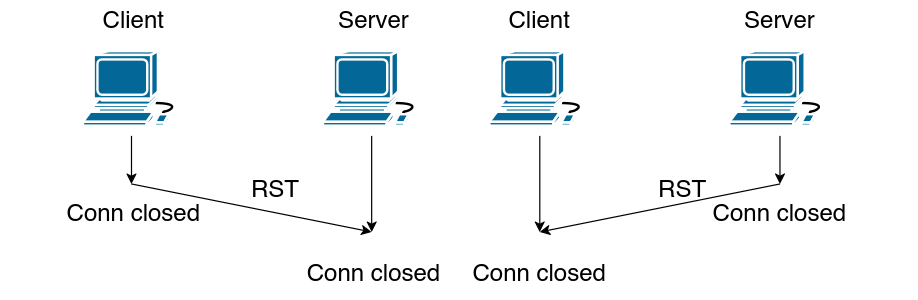
\includegraphics[width=1.2\linewidth]{Images/livello_trasporto/RST.png}
        \caption{Interruzione di una connessione.}
    \end{minipage}
\end{figure}

\section{Affidabilotà nel protocollo TCP}
Ci sono diversi meccanismi per garantire affidabilità in modo trasparente rispetto al processo applicativo:
\begin{itemize}
    \item \textbf{ACK.}
    \item \textbf{Timeout.}
    \item \textbf{Ritrasmissione.}
\end{itemize}
Ogni trasmissione riuscita viene \textbf{confermata} dall'host ricevente.Se l'host mittente non riceve una conferma entro il \textbf{timeout}, il mittente ritrasmette i \textbf{dati}.

\subsection{Stima del Timeout}
La stima del timeout viene fatto usando l'\textbf{RTT (Round Trip Time)}. Il valore è molto importante calcolarlo bene, perchè se troppo basso si rischia di dover inviare il segmento più volte, se troppo alto, invece, si ha una lenta risposta ai segmenti persi. In generale, il timeout deve essere dell'RTT.
Ci sono due modi per misusare il Round Trip Time:
\begin{enumerate}
    \item \textbf{SamlpleRTT:} misura il tempo dall'invio del segmento alla ricezione dell'ACK, varia più volte dinamicamente.
    \item \textbf{EstimatedRTT:} media pesata per sapere l'RTT a un tempo \textbf{t}: 
    \[
        \text{EstimatedRTT}(t) = (1 - \alpha) \cdot \text{EstimatedRTT}(t-1) + \alpha \cdot \text{SampleRTT}(t)
    \]
    Dove, dato un numero $n$ di casi:
    \[
        \alpha = \frac{1}{n+1}
    \]
\end{enumerate}
Attualmente, il \textbf{timeout} è calcolato usando l'EstimatedRTT e un piccolo margine:
\[
    \text{Timeout}(t) = \text{EstimatedRTT}(t) + Dev(t)
\]
Dove:
\[
    Dev(t) = (1-\alpha)Dev(t-1) \space + \space \alpha \cdot |\text{SampleRTT}(t)-\text{EstimatedRTT(t)}|
\]

\newpage
\section{Gestione del Buffer TCP}
TCP, essendo parte del Sistema Operativo e non del layer applicativo, deve riuscire a gestire tutte gli eventi asincroni che accadono. Infatti, il protocollo TCP non sa quando un processo vorrà inviare i dati o quando li vorrà ricevere. Per questo si inseriscono temporaneamente i dati dentro un \textbf{buffer}.

\begin{boxDef}
\textbf{\textcolor{brown}{Alcune definizioni:}}
\begin{itemize}
    \item \textbf{RTT:} tempo di un segmento per arrivare a destinazione e tornare indietro.
    \item \textbf{Tempo di propagazione ($\text{T}_p$):} $\frac{\text{RTT}}{2}$.
    \item \textbf{Utilizzo (U):} percentuale di utilizzo delle risorse.
    \item \textbf{Frequenza di Trasmissione ($\text{T}_r$).} 
    \item \textbf{Packet Lenght:} $L(pkt)$.
    \item \textbf{Tempo di trasmissione di un pacchetto (TT):} $\frac{L(pkt)}{\text{T}_r}$.
    \item \textbf{Tempo di trasferimento di un segmento(T):} T = $[\frac{\text{RTT}}{2} + L(pkt)] + \frac{\text{RTT}}{2}$
\end{itemize}
\end{boxDef}
I buffer servono per passare da un meccanismo \textbf{Stop-and-Wait} a uno in \textbf{pipeline}. Devono essere implementati sia dal lato del mandante che del destinatario, insieme a protoccoli \textbf{Sliding Windows} per sapere quanti pacchetti mandare senza ricevere il loro ACK.

\begin{figure}[!htb]
    \centering
    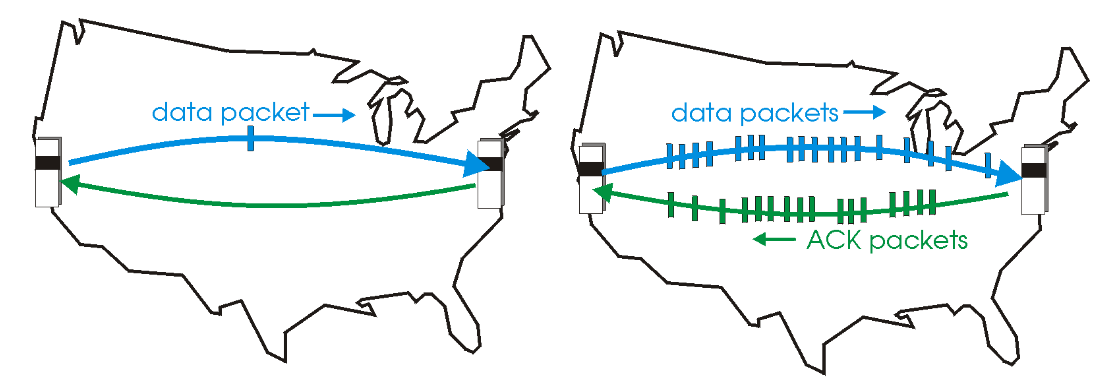
\includegraphics[width=0.8\linewidth]{Images/livello_trasporto/Stop-and-Wait.png}
    \caption{Protocolli Stop-and-Wait e con Pipeline.}
\end{figure}

\begin{figure}[!htb]
    \centering
    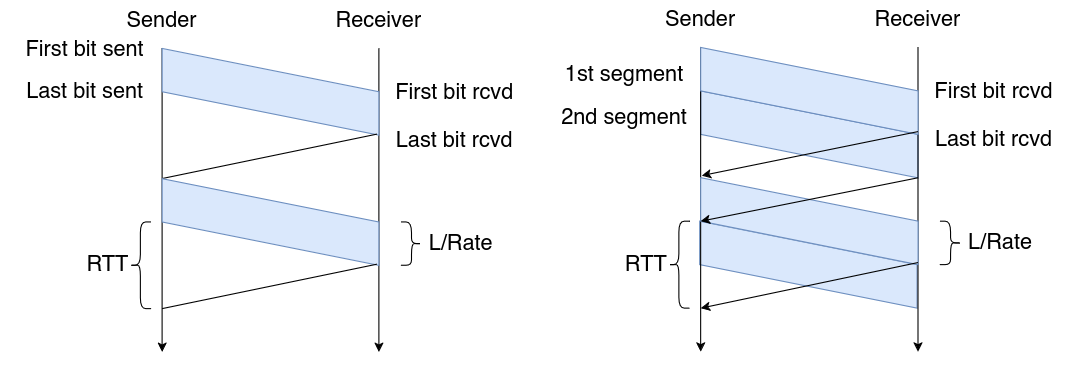
\includegraphics[width=0.8\linewidth]{Images/livello_trasporto/Pipeline.png}
    \caption{Protocolli Stop-and-Wait e con Pipeline.}
\end{figure}

\newpage
\subsection{Sliding Windows}
Il mittente assegna a ciascun segmento un numero di sequenza \textbf{segment\_no} nelll'intervallo $[0, 2^{32} - 1]$.
\begin{center}
    \begin{minipage}{.45\linewidth}
        \begin{boxDef}
        \textbf{\textcolor{brown}{Mandante}} \\
        In ogni momento, il mittente mantiene una sliding window sugli indici di segmento e solo quelli all'interno della finestra possono essere trasmessi. La dimensione della finestra utile del mittente è controllata dal destinatario. Usa tre variabili:
            \begin{itemize}
                \item \textbf{Sender Window Size (SWS):} il massimo di segmenti che può mandare senza ricevere un ACK.
                \item \textbf{Last ACK Received (LAR):} numero di sequenza dell'ultimo ACK ricevuto.
                \item \textbf{Last Segment Send (LSS):} numero di sequenza dell'ultimo segmento inviato.
            \end{itemize}
        \textbf{NB:} \[\text{LAS} - \text{LSR} \ge \text{RWS}\]
        \end{boxDef}
    \end{minipage}
    \begin{minipage}{.45\linewidth}
        \begin{boxDef}
        \textbf{\textcolor{brown}{Ricevente}} \\
        In qualsiasi momento, il destinatario mantiene una sliding window sugli indici dei segmenti ricevuti. La dimensione della finestra e le modalità di gestione dipendono dall'algoritmo utilizzato. Usa tre variabili:
            \begin{itemize}
                \item \textbf{Receive Window Size (RWS):} indica il numero massimo di segmenti fuori sequenza che può accettare.
                \item \textbf{Largest Accetable Segment (LAS):} numero di sequenza più grande che può accettare. 
                \item \textbf{Last Segment Received (LSR):} numero di sequenza dell'ultimo segmentoricevuto in ordine.
            \end{itemize}
        \textbf{NB:} \[\text{LSS} - \text{LAR} \ge \text{SWS} \]
        \end{boxDef}
    \end{minipage}
\end{center}

\begin{figure}[!htb]
    \begin{minipage}{.47\linewidth}
        \centering
        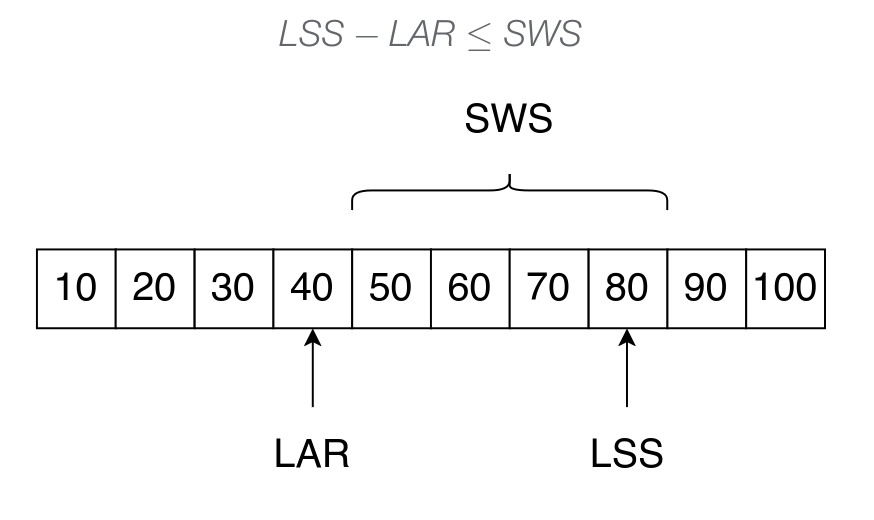
\includegraphics[width=0.8\linewidth]{Images/livello_trasporto/Mandante.png}
        \caption{Chiusura pulita di una connessione.}
    \end{minipage}
    \begin{minipage}{.47\linewidth}
        \centering
        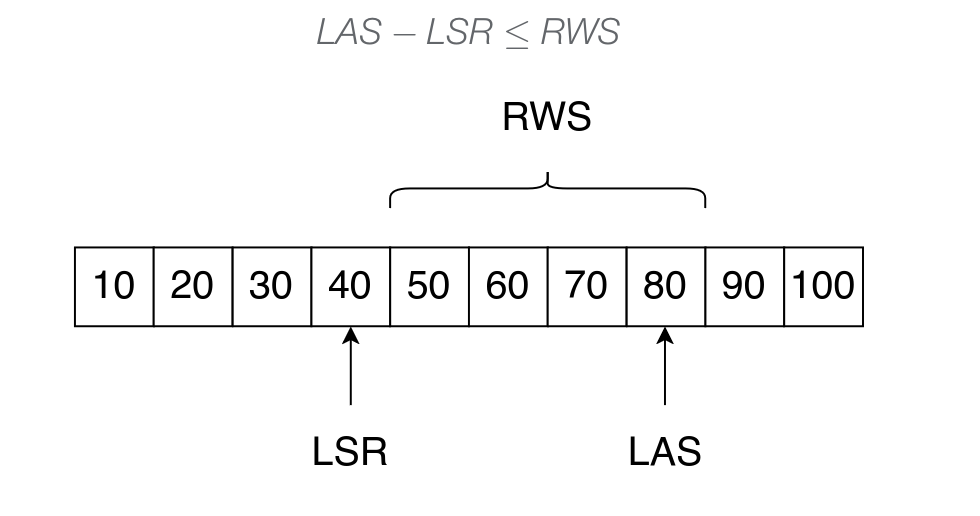
\includegraphics[width=0.9\linewidth]{Images/livello_trasporto/Ricevente.png}
        \caption{Interruzione di una connessione.}
    \end{minipage}
\end{figure}

\subsection{Flow Control}
L'obiettivo è non far inviare al mandante più dati di quelli che il buffer del destinatario può contenere. Il ricevitore comunica esplicitamente al mittente la quantità di spazio libero nel buffer di ricezione TCP e varia dinamicamente, quindi ogni segmento ACK comunica al mittente il numero massimo di byte ricevibili.

\begin{figure}[!htb]
    \centering
    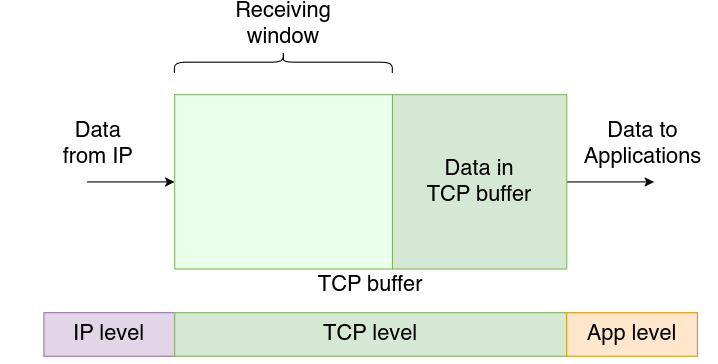
\includegraphics[width=0.6\linewidth]{Images/livello_trasporto/FlowControl.png}
    \caption{Buffer TCP.}
\end{figure}

L'ACK contiene due informazioni:
\begin{enumerate}
    \item Quanti byte ha ricevuto il recipiente.
    \item Quanti byte può ancora ricevere in quel momento.
\end{enumerate}

\[
\textbf{Advertised Window} = \text{MaxRcvBuffer} -((\text{NextByteExpected} - 1) - \text{LastByteRead})
\]

\[
\textbf{EffectiveWindow} = \text{AdvertisedWindow} - (\text{LastByteSent} - \text{LastByteAcked})
\]

Quando il mandante riceve $\textbf{Advertised Window} = 0$, teoricamente non può più mandare dati e per questo non riesce a capire quando può ricominciare a mandare dati. La soluzione nel protocollo TCP è mandare costantemente mandare un segmento con un byte di dato.

\subsection{Congestion Control}
La congestione in una rete può causare diversi problemi, come la perdita di pacchetti oppure tempi di delay molto elevati.
Ci sono due modi per approcciarsi alla gestione della congestione:
\begin{enumerate}
    \item \textbf{Controllo end-to-end:} approccio usato dal protocollo TCP, non viene gestito dalla rete, ma si guardano i pacchetti persi e il tempo di delay.
    \item \textbf{Controllo di rete:} i router dicono ai nodi terminali lo stato della congestione della rete.
\end{enumerate}

\begin{figure}[!htb]
    \centering
    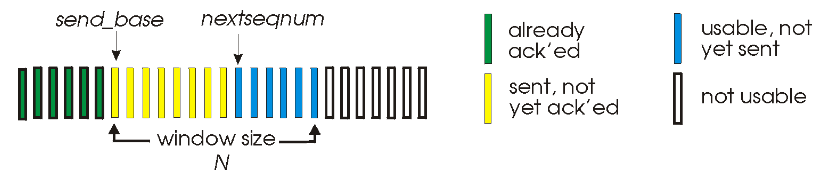
\includegraphics[width=0.8\linewidth]{Images/livello_trasporto/WindowSize.png}
    \caption{Dimensione della finestra nel TCP.}
\end{figure}

Le prestazioni nel protocollo TCP vengono misurate tramite il \textbf{Throughput}:
\[
\textbf{Throughput} = \frac{w \space\cdot MSS}{RTT}
\]
Dove $w$ è il numero di segmenti della finestra.
Esistono diversi algortimi per evitare la congestione della rete:

\subsubsection{Slow Start}
Inizia con la dimensione della finestra di congestione pari a 1 e poi in modo esponenziale aumenta fino al threshold.

\begin{bashbox}
ffor each ACK segment do
    CW++
    if timeout OR CW > threshold then
        break
\end{bashbox}


\subsubsection{Tahoe Algorithm}
Cresce in modo esponenziale fino al threshold, poi incrementa di 1.

\textbf{\{Slow start ended, CW $\ge$ threshold\}}
\begin{bashbox}
iif not loss then
    for all ACK segment
        CW++
else
    threshold = CW/2
    CW = 1
    do slow start
\end{bashbox}


\subsubsection{Reno Algorithm}
Controlla due tipi di errore:
\begin{enumerate}
    \item \textbf{Timeout:} riduce la finestra di congestione a 1.
    \item \textbf{Tre ACK duplicati:} riduce la finestra di metà.
\end{enumerate}

\textbf{\{Slow start ended, CW $\ge$ threshold\}}
\begin{bashbox}
iif not loss then
    for all ACK segment 
        CW++
else
    threshold = CW/2
    if Loss detected by timeout then
        CW = 1
        do slow start
    if loss detected by triple ACK then
        CW = CW/2
\end{bashbox}
Reno, in confronto a Tohoe, ha una recupero molto più veloce, ma ormai, entrambi sono obsoleti.

\subsubsection{Vegas Algorithm}
Il timeout è basato sull'RTT e ha un contatore che controlla ogni pacchetto.

\begin{bashbox}
xx(t) = [WSize(t) - WSize(t-1)] / [RTT(t) - RTT(t-1]
if x(t) > 0
    CW = CW - CW/8
else
    CW = CW + MSS
\end{bashbox}
Se aumenta la congestione aumenta pure l'RTT e viceversa. La finestra di congestione cambia ogni $2 \cdot \text{RTT}$.

\subsubsection{BIC (Binary Increase Congestion)}
Mantiene 4 valori diversi di finestre di congestione:
\begin{enumerate}
    \item \textbf{Attuale.}
    \item \textbf{Massima.}
    \item \textbf{Minima.}
    \item \textbf{Prevista (valore fra massimo e minimo).}
\end{enumerate}
Nello specifico: 
\begin{enumerate}
    \item Quando la differenza tra la finestra minima e quella massima è ampia, si ricorre a una crescita aggressiva della finestra (\textbf{incremento additivo}).
    \item Quando la finestra corrente raggiunge quella prevista senza errori, la finestra minima diventa quella prevista.
    \item In caso di errore, la finestra massima assume il valore della finestra corrente. La finestra corrente si riduce al nuovo valore minimo.
    \item Man mano che le finestre minime e massime si restringono, la ricerca diventa meno aggressiva.
\end{enumerate}

\subsubsection{CUBIC}
Evoluzione di BIC, mantiene la sua stabilità e scalabilità, ma aumenta la fairness. Infatti, la dimensione della finestra di congestione dipende la tempo e non dall'RTT.

\subsection{Buffer Bloating}
Problema regolato dalla presenza di buffer molto grandi nella rete, tipicamente di dimensioni variabili. Si verifica in presenza di trasferimenti di dati di lunga durata e dalla presenza di più flussi TCP simultanei. Quando i buffer sono pieni, l'RTT è così elevato che il timeout per la perdita di pacchetti rallenta l'intervento del controllo della congestione. Il risultato è il calo del throughput a causa dei ritardi e un elevato tasso di perdita di pacchetti.
Esistono alcune proposte per risolvere questo problema come:
\begin{itemize}
    \item \textbf{CoDel Algortihm (Controlled Delay)} come algoritmo di AQM (Adaptive Queue Management) per gestire la grandezza dei buffer in modo dinamico per più flussi TCP.
    \item \textbf{Google SPDY.}
    \item \textbf{HTTP/2.}
\end{itemize}
